\documentclass[11pt]{article}
\usepackage{color}
\usepackage{authblk}%allows footnote format for authors
\usepackage[letterpaper, margin=1in]{geometry} %package that allows changes in margins and header/footers
\usepackage[numbers,sort]{natbib}
\usepackage{amsmath}
\usepackage{rotating}
\usepackage{adjustbox}
\usepackage[english]{babel}
\usepackage{colortbl}
\usepackage{booktabs}
\usepackage{tabularx}
\usepackage[x11names,dvipsnames,table]{xcolor}
\usepackage{array}
\newcolumntype{G}[1]{>{\raggedright\let\newline\\\arraybackslash\hspace{0pt}}m{#1}}
\bibliographystyle{ieeetr}
\newcommand{\mbh}[1]{\textcolor{orange}{ \emph{\scriptsize  #1}} } %creating command for Matt's comments
\newcommand{\lwang}[1]{\textcolor{red}{ \emph{\scriptsize  #1}} } %creating command for Li's comments
\newcommand{\gmj}[1]{\textcolor{blue}{ \emph{\scriptsize  #1}} } %creating command for Garrett's comments

\title{Review: The Prevalence of Adaptive Introgression in Crop Histories}

\author[1]{Authors: Garrett M. Janzen}%author information
\author[1]{Li Wang}
\author[1,*]{Matthew B. Hufford}
\affil[1]{Department of Ecology, Evolution, and Organismal Biology, Iowa State University, Ames, Iowa, USA}
\affil[*]{Correspondence: mhufford@iastate.edu (M.B. Hufford)}
\date{}

\begin{document}

\maketitle

Plant domestication is often conceptualized as a geographically constrained process, with crops originating from a wild progenitor within one or more defined centers followed by expansion to the modern-day range of cultivation \cite{Harlan1992}.
However, archaeological and genetic evidence are beginning to reveal that, in many cases, domestication has been temporally protracted and geographically diffuse \cite{Meyer2016, Wang2017, Fuller2014}.
An additional important aspect of the emerging complexity of domestication is the occurrence of beneficial gene flow from locally adapted wild relatives to crops during their expansion following initial domestication.
It is this adaptive introgression that is the subject of this review.

Adaptive introgression has three components: hybridization between differentiated taxa, backcrossing to one of the parents, and selection on recombinant genotypes with progressively diminished linkage drag \cite{barton2001role}.
In domesticated species, adaptive introgression would consist of crop-wild hybrids backcrossing to a crop followed by increase in frequency of adaptive wild alleles in the crop and selection against undesirable wild background.
To date, the literature on crop-wild gene flow has largely focused on the risk of transgene introgression from domesticated crops into wild relatives (for a review, \cite{stewart2003transgene}) and on modern plant breeding efforts to introgress desired traits from wild relatives (for a review, \cite{Dempewolf2017}).
The history of natural and potentially adaptive introgression of wild alleles into domesticated crops over evolutionary timescales has received considerably less attention.
However, new tools and methods have recently been employed to detect genome-wide patterns of introgression, granting new insights into the prevalence of adaptive introgression in crop histories.
Emerging results from these studies suggest there is a need to expand our conception of domestication to encompass the broadening of the genetic base of crops that occurred through adaptive gene flow from newly encountered wild relatives during post-domestication expansion.

In this review, we: 1) briefly describe recently developed methods for detecting introgression, 2) present case studies suggesting wild-to-crop introgression has conferred local adaptation, 3) consider how introgression bears upon fundamental questions of domestication, and 4) describe some key questions regarding crop adaptation that is mediated by gene flow from wild relatives.


\section*{Introgression methods and their application}


The decreasing cost of genome-wide resequencing and availability of reduced-representation genotyping (\emph{e.g.}, GBS and RAD-Seq), combined with new analytical methods (\textbf{Table 1}), has facilitated the comprehensive study of introgression across a broad spectrum of domesticated species.
The methods reviewed here do not include those marginally estimating introgression\slash migration rate as a component of demographic history (\emph{e.g.}, Approximate Bayesian Computation (ABC) \cite{beaumont2002}, diffusion approximations for demographic inference ($\delta a\delta i$) \cite{gutenkunst2009}, isolation with migration models \cite{hey2004}, and methods utilizing the sequentially Markovian coalescent (\emph{e.g.}, PSMC) \cite{li2011}). 
Rather, we focus on three broad categories of methods that explicitly identify introgressed genomic segments based on the extent of differentiation, patterns of nucleotide/haplotype sharing, and phylogenetic relationships.

First, introgressed segments are expected to show low differentiation from their source population.
The $F_{st}$ and $d_{XY}$ statistics and their derivates including $G_{min}$ \cite{geneva2015} and $RND_{min}$\cite{rosenzweig2016} gauge differentiation. 
The former two statistics are insensitive to rare migrants and therefore lack power to detect recent introgression, while the latter two overcome this limitation.
Additionally, $RND_{min}$ accounts for variable mutation rate, which is detected based on branch length to an outgroup \cite{rosenzweig2016}.
These statistics have been further developed by adding differentiation between both non-admixed ($A$) and admixed populations ($B$) and a source population ($C$) \cite{racimo2016}. 
For example, the $U_{A,B,C(w,x,y)}$ statistic summarizes the number of sites where an allele at frequency $y$ in the source population ($C$) has a frequency higher than $x$ in the admixed population ($B$) and lower than $w$ in the non-admixed population ($A$).
A similar statistic, $Q95_{A,B,C(w,y)}$, sets a hard cutoff at the $95^{th}$ percentile of allele frequency in the admixed population (B) \cite{racimo2016}.
Further modifications have allowed specification of more than one source population (see details in \cite{racimo2016}).
Since differentiation-based methods can be calculated site-by-site, high-density, genome-wide data are not necessarily required.
However, accuracy of introgression estimates is improved with more comprehensive data.
 
Second, local ancestry deconvolution assigns genomic regions to various source populations based on patterns of allele or haplotype sharing \cite{schraiber2015}. 
One form of ancestry deconvolution utilizes a hidden Markov model to evaluate ancestry across admixed genomes through comparison to reference, non-admixed individuals (\emph{e.g.}, HAPMIX \cite{Price2009}). 
Another clusters admixed populations with reference samples using a sliding-window approach (\emph{e.g.}, PCAdmix \cite{brisbin2012pcadmix} and LAMP \cite{sankararaman2008}).
And finally, introgression can be detected through ancestry deconvolution by using a Bayesian model \cite{pritchard2000} in which deviations from Hardy-Weinberg equilibrium are minimized through creation of genetic groups (\emph{e.g.}, fineSTRUCTURE \cite{Lawson2012}).
Ancestry deconvolution methods are better suited to high-density marker or whole genome sequencing data given the intent to assign ancestry genome-wide.

Phylogenetic relationships are evaluated and applied to introgression detection using the ABBA-BABA statistic (also known as the D-statistic) and related metrics.
These statistics make inferences regarding introgression based on genomic patterns of derived variants that are shared between populations or species.
While the D-statistic is best suited to detection of introgression at the genome level, elaborations of the D-statistic including $\hat{f_{d}}$ \cite{martin2015} and $D_{\textrm{FOIL}}$ tests \cite{pease2015} are capable of localizing introgression to specific chromosomal regions. 
The former is quite similar to the D-statistic but uses allele frequencies from each population/species, and the latter can identify donor and recipient lineages of introgression in a more complex, five-taxon phylogeny.
Like differentiation methods, phylogeny-based detection of introgression can be employed using low-density data.
However, because these methods require knowledge of whether an allele is ancestral or derived, data from a sufficiently diverged outgroup must also be included in analyses.

Application of these approaches, in combination with population genetic statistics to detect selection, suggest that introgression can play an adaptive role.
For example, based on sequence divergence methods, introgression has been detected in \emph{Mimulus} (\emph{i.e.}, monkeyflower) species and appears to play a role in both adaptation to pollinator preference and speciation \cite{Stankowski2015}.
Likewise, the HAPMIX ancestry deconvolution method was applied by Jeong et al. \cite{jeong2014} to detect introgression in human populations from the Nepalese Sherpa to Tibetans at loci controlling high altitude adaptation (reviewed in \cite{Racimo2015}).
Finally, the ABBA-BABA statistic has revealed introgression at wing coloration loci conferring M\"{u}llerian mimicry across butterfly species \cite{heliconius2012}.

\begin{table}[h]

\rowcolors{2}{white}{gray!25}
\begin{center}
\caption{List of recently developed methods for detecting introgression and examples of their use in empirical studies.} \label{tab:tools}
\begin{tabularx}{\textwidth}{llll}
\\\toprule  
\rowcolor{white}
{\bf Methods}	& {\bf Data Type } &	{\bf References} &  {\bf Applications } \\ \midrule

\rowcolor{gray!25}
{\emph{\bf Divergence}} &   &   &   \\
\rowcolor{gray!25}
Gmin &	biallelic SNP	&  \cite{geneva2015}	 &  \cite{kingan2015}\\
\rowcolor{gray!25}
RNDmin	& phased haplotype	& \cite{rosenzweig2016} &  \cite{roda2017} \\
\rowcolor{gray!25}
$U_{A,B,C(w,x,y)}$ and $Q95_{A,B,C(w,y)}$ & biallelic SNP & \cite{Racimo2015} & \cite{sams2016} \\

\rowcolor{white}
{\emph{\bf Ancestry Deconvolution}} &   &   &   \\
\rowcolor{white}
Hapmix	& phased haplotype; reference panel		& \cite{Price2009}	&  \cite{Hufford2013} \\ 
\rowcolor{white}
RASPberry &	phased haplotype &	\cite{wegmann2011}	 & \cite{christe2016} \\
\rowcolor{white}
MultiMix & phased/unphased genotype; reference panel &	\cite{churchhouse2013} &	\cite{eyheramendy2015} \\
\rowcolor{white}
PCAdmix	 & phased haplotype	 & \cite{brisbin2012pcadmix}	 &  \cite{moreno2014genetics} \\
\rowcolor{white}
LAMP  &	phased haplotypes; reference panel	 & \cite{sankararaman2008}	 & \cite{patterson2012} \\

\rowcolor{gray!25}
{\emph{\bf Phylogenetic Relationship}} &   &   &   \\
\rowcolor{gray!25}
ABBA-BABA/D-statistics	 & biallelic SNP  &	\cite{durand2011}	 &  \cite{heliconius2012} \\
\rowcolor{gray!25}
fd statistic &	biallelic SNP &	\cite{martin2015}  &	\cite{zhang2016genome} \\ 
\rowcolor{gray!25}
five taxon D statistics	& biallelic SNP	&  \cite{pease2015}	& \cite{fontaine2015} \\

\end{tabularx}
\end{center}
\end{table} 



\section*{Crop adaptation through introgression}

As comprehensive genetic analyses of crops and their wild relatives have become feasible across their geographic ranges, evidence for substantial wild-to-crop introgression has been discovered in some of the world's most important crops (\textbf{Table 2}).
Below we present a summary of findings from maize, barley, rice, and potato, four systems in which introgression from wild relatives appears to have played an adaptive role.
All four of these crops were domesticated in defined centers and have subsequently expanded to much broader distributions, a migration that brought them into contact with new populations of wild relatives (Figure \ref{fig:map}).

\begin{figure}[h]
	\centering
	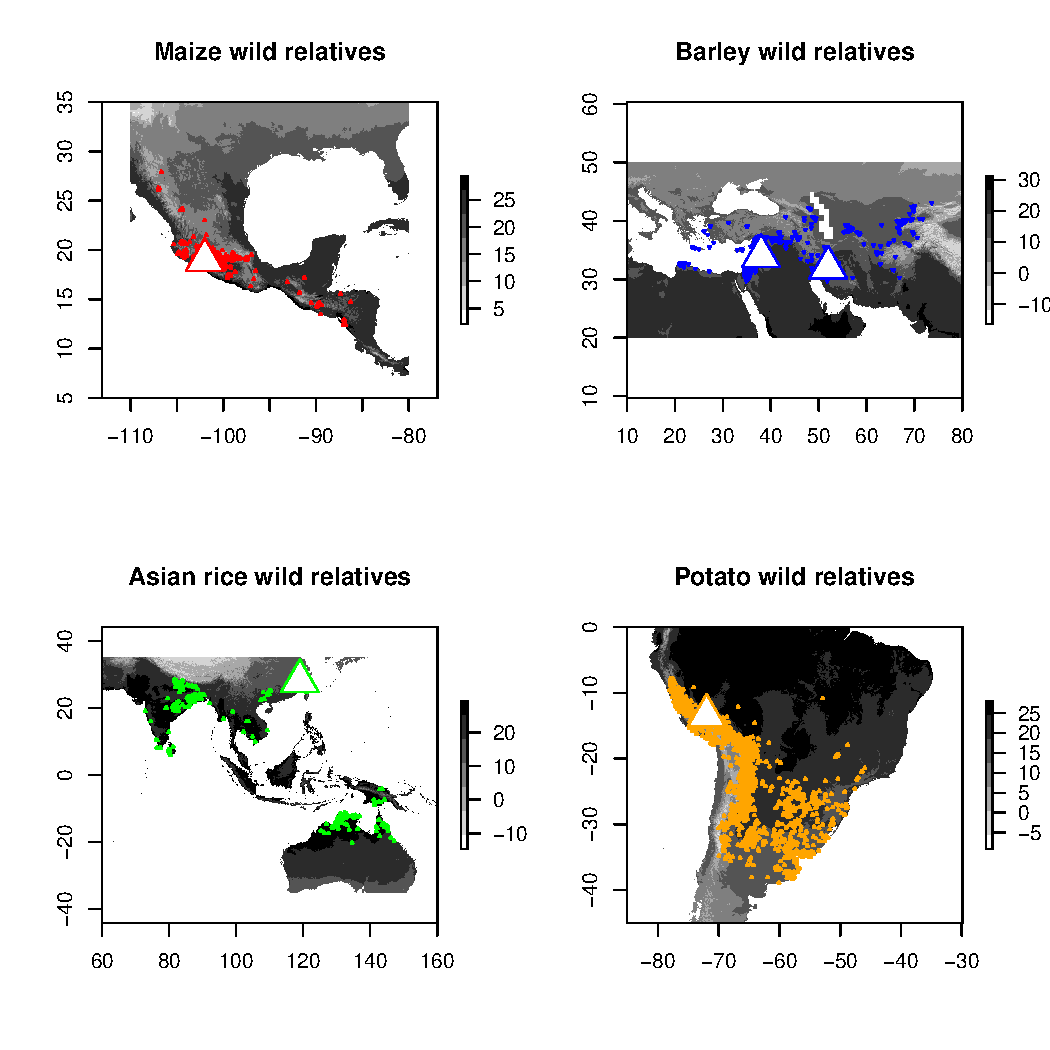
\includegraphics[width=15cm]{temperature_plot_degC.pdf}
	\caption{Map of the natural ranges of wild relatives of four domesticated crops, overlayed with average annual temperature. Approximate domestication center for each crop is denoted by a triangle}
	\label{fig:map}
\end{figure}


\begin{enumerate}
\item{Maize:}

The relationship between maize (\emph{Zea mays} ssp. \emph{mays}) and the teosinte \emph{Zea mays} ssp. \emph{mexicana} (hereafter, \emph{mexicana}) offers a prime example of adaptive wild-to-crop introgression.
Maize was domesticated from \emph{Zea mays} ssp. \emph{parviglumis} (hereafter, \emph{parviglumis})  approximately 9,000 BP in the lowlands of the Balsas River Valley in Mexico \cite{matsuoka2002single}.
From this domestication center, maize spread into the highlands of the Mexican Central Plateau, where it came into sympatry with \emph{mexicana}.
Introgression from \emph{mexicana} to maize in the Central Plateau has been reported based on both morphological \cite {wilkes1977} and molecular \cite{vanHeerwaarden2011, doebley1987} data.
However, Hufford et al. \cite{Hufford2013} first localized \emph{mexicana} introgression to chromosomal regions and provided evidence that it was likely adaptive.
The authors identified nine genomic regions in several maize populations which consistently showed evidence of \emph{mexicana} introgression based on ancestry deconvolution methods including HAPMIX (Figure \ref{fig:introgressionMaize}).
These introgressed segments overlapped with QTL that had previously been found to control anthocyanin content and leaf macrohairs \cite{lauter2004}, traits known to be adaptive at high elevation.
In a growth chamber experiment, the authors demonstrated that maize populations with \emph{mexicana} introgression showed greater plant height (a proxy for fitness) under highland environmental conditions than populations that lacked introgression.
Height differences were not detected under lowland conditions, providing further evidence of local adaptation.


Populations of \emph{mexicana} cannot be found outside the highlands of Mexico, yet maize has colonized and adapted to high elevation in a number of other regions.
Wang and co-authors \cite{Wang2017} employed the ABBA-BABA and $\hat{f_{d}}$ statistics to evaluate if maize with \emph{mexicana} introgression was transferred to other highland regions or whether highland adaptation was obtained \emph{de novo} outside of Mexico.
Overall, analyses revealed that  \emph{mexicana} introgression was pervasive in maize from Mesoamerican high elevation regions (the highlands of Mexico, Guatemala, and the southwestern United States), but more distant high elevation regions (\emph{e.g.,} the Andes) showed no \emph{mexicana} ancestry.
Maize from the lowlands of northern South America appears to have been derived from Mesoamerican lowland maize and high elevation adaptation in Andean maize likely occurred \emph{de novo} from this genetic base.


\begin{figure}[h]
	\centering
	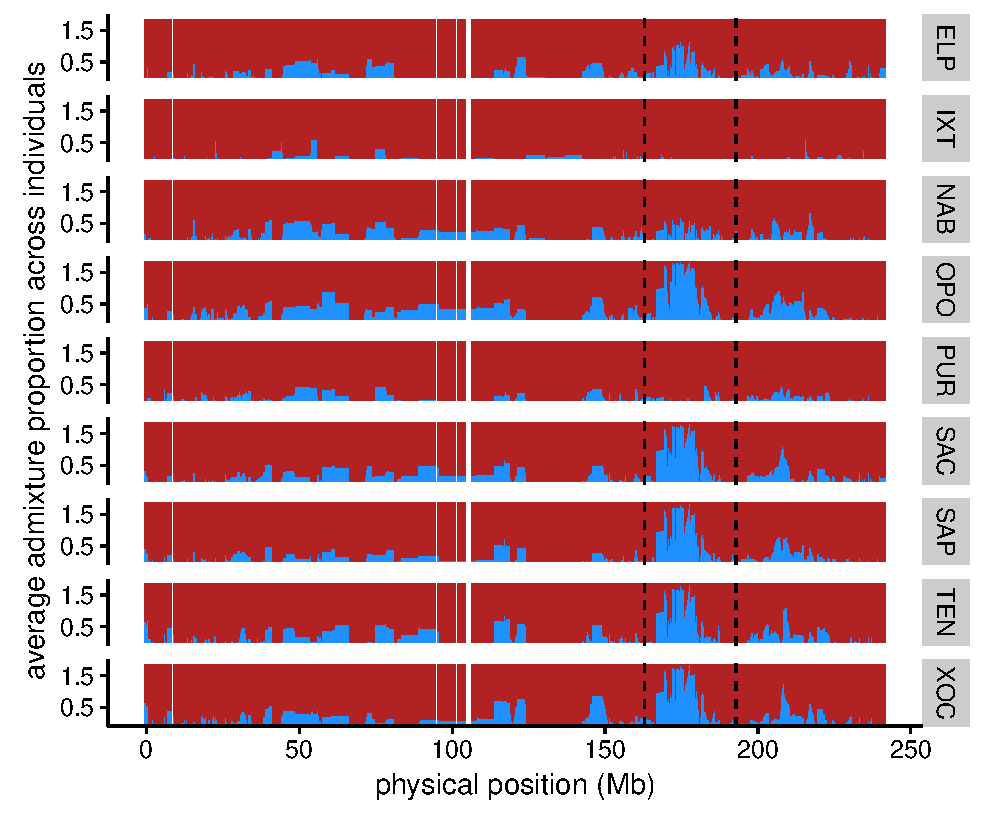
\includegraphics[width=12cm]{./FigsAndTables/Figure1new}
	\caption{Hapmix vectors indicating introgression level from \emph{mexicana} to Mexican highland maize on chromosome 4. Data adopted from Hufford et al. \cite{Hufford2013}. ELP: EL Porvenir; IXT: Ixtlan ; NAB: Nabogame; OPO: Opopeo; PUR: Puruandiro; SAC: Santa Clara; SAP: San Pedro; TEN: Tenango del Aire; XOC: Xochimilco. Insets show the phenotypic differences between lowland (red) and highland (blue) maize stems. The black bar indicates one of the QTLs for macrohairs and pigment density in Lauter et al. \cite{lauter2004}.}
	\label{fig:introgressionMaize}
\end{figure}

\item{Barley:}

Barley (\emph{Hordeum vulgare} subsp. \emph{vulgare}) was domesticated from wild subsp. \emph{spontaneum} roughly 8,000 to 10,000 BP.
Modern barley is most likely the result of multiple domestication events across the Middle East and Asia \cite{azhaguvel2007phylogenetic}.
There is clear evidence of one domestication event of barley from the wild subsp. \emph{spontaneum} in the Fertile Crescent \cite{badr2000origin, Morrell2007}, and many have supported an additional eastern center of barley domestication from subsp. \emph{spontaneum} var. \emph{agriocrithon} \cite{Morrell2007}, possibly Tibet \cite{dai2012tibet}.
However, recent research from Pourkheirandish and colleagues \cite{pourkheirandish2018elucidation} suggests that the putative wild Tibetan progenitor \emph{agriocrithon} is a misidentified intercultivar hybrid of domesticated 6-row landraces, which they deem \emph{pseudo-agriocrithon}, as opposed to \emph{eu-agriocrithon}, which are six-rowed wild relatives derived from two-rowed \emph{ssp. spontaneum}.
The non-brittle rachis mutations (\emph{btr1} and \emph{btr2}) appear to have arisen in populations from the Levant, whereas the two most common of four alleles conferring 6-rowed spike morphology (\emph{vrs1.a1} and \emph{vrs1.a4}) originated in \emph{eu-agriocrithon} populations in Central Asia (Turkmenistan and Uzbekistan, respectively).
These two key barley domestication traits were combined when \emph{vrs1.a1} and \emph{vrs1.a4} introgressed from \emph{eu-agriocrithon} into cultivated barleys in the Levant.

Presently, the distribution of subsp. \emph{spontaneum} stretches from the eastern Mediterranean through the Middle-East to west-central Asia, spanning clines in temperature, precipitation, soil type, and altitude \cite{Morrell2007}.
Cultivated barley is found throughout much of the \emph{spontaneum} distribution and barley-\emph{spontaneum} hybrids are fertile and commonly found when these taxa co-occur.

Poets and co-authors \cite{Poets2015} recently investigated the range-wide contribution of wild barley to landraces, assessing both genome-wide and geographical patterns of introgression.
This study identified several lines of evidence consistent with wild introgression aiding the expansion and adaptation of domesticated barley.
Using ancestry deconvolution methods, the authors identified genomic regions of shared ancestry linking particular landraces to numerous wild relative populations.
These results suggested landraces may have received wild introgression on a continual basis during post-domestication expansion.
However, barley landraces also showed an excess of ancestry from nearby wild relatives, indicating a prevalence of local and potentially adaptive gene flow.
Limited admixture linkage disequilibrium and small tracts of identity by state suggest substantial recombination has occurred since initial crop-wild hybridization and that even locally introgressed chromosomal regions are ancient, perhaps dating to the early expansion of barley post-domestication.
While these results are consistent with adaptive introgression, wild barley haplotypes have yet to be definitively linked to specific adaptations in landraces post-domestication.

%"The best current hypothesis holds that both vrs1.a1 and vrs1.a4 were introgressed from eu-agriocrithon into other wild barley genotypes and then outcrossed to cultivated barley (Figure 1)"

%"The proposal here is that vrs1.a1 and vrs1.a4 emerged in agriocrithon before they were introgressed into ssp. vulgare (Figure 1)."

%"The origin of two alleles (vrs1.a2 and a3) was previously shown (Komatsuda et al., 2007) to involve single mutations at the vrs1 locus that changed the domesticated two-rowed to six-rowed phenotype (Figure 1)."

%"Both vrs1.a1 and vrs1.a4 arose in Central Asia, some 2500 km distant from the site of emergence of non-brittle rachis. The occurrence of six-rowed types among wild barley implies that the six-rowed allele pre-dates domestication, when early farmers still relied on ssp. spontaneum. This time line agrees, in part at least, with the notion that six-rowed cultivated barley was derived from agriocrithon (Aberg, 1938). The non-brittle rachis trait represents a strong genetic bottleneck, and its geographical origin lies far from that of eu-agriocrithon, clearly implying that eu-agriocrithon could not have been the immediate ancestor of the non-brittle barleys that were donors of vrs1.a1 and vrs1.a4 to cultivated barley."

\item{Potato}

Modern potato (\emph{Solanum tuberosum}) was likely domesticated approximately 6,000-10,000 BP in southern Peru in sympatry with several wild relatives.
The exact progenitor has remained in question for some time \cite{spooner2005single, pickersgill1977origins, hawkes1988evolution}, but a distance-based phylogeny constructed using genotypic data from a \emph{Solanum} diversity panel recently identified \emph{S. candolleanum} as the most probable progenitor \cite{hardigan2015taxonomy}.
The lack of clarity regarding a progenitor has been due, in part, to extensive post-domestication hybridization between potato and a number of related species.

While potatoes are primarily propagated clonally, farmers do at times promote sexual reproduction for improvement of the crop and development of new cultivars \cite{quiros1992increase}.
Close proximity of domesticated potatoes and wild relatives, active hybridization, and local selection pressure favoring wild haplotypes across a diverse range of biotic and environmental conditions have likely fostered an expansion of genetic diversity within potatoes subsequent to domestication \cite{brush1995potato}.
The prevalence of wild introgression was recently clarified in a broad survey of potato diversity by Hardigan and colleagues \cite{hardigan2017genome}.
These authors discovered that both diploid and tetraploid domesticates had received extensive introgression from more than ten species of wild \emph{Solanum}, with a continued broadening of the genetic base of potato as it spread away from its Peruvian origin.
In certain cultivars, wild ancestry was estimated at upwards of 30\%.
Genes located within these introgressed regions were more likely to be highly-expressed and stress-inducible, and contained loci related to disease resistance, drought tolerance, and heat tolerance, suggesting introgression conferred adaptations critical to survival, possibly facilitating tolerance for new environmental pressures during range expansion \cite{hardigan2017genome}.
\end{enumerate}


The four crop systems described in detail here represent particularly compelling examples of putatively adaptive wild introgression.
However, given their similar histories, many additional crops have likely benefited from wild-to-crop gene flow during post-domestication expansion (\textbf{Table 1}).
Across these four cases studies, potential generalities can be observed.
Data thus far indicate that wild introgression is often local or regional in its extent, but that, in certain cases (\emph{e.g.}, \emph{mexicana} haplotypes detected in maize landraces from the Guatemalan or southwestern U.S. highlands), newly introgressed wild haplotypes can be disseminated more broadly.
Additionally, when functional information is evaluated, as in the maize and potato studies, introgression has been found to occur at loci conferring adaptation to novel conditions not found in a crop's center of origin.
Beyond these observations associated with post-domestication adaptation, pervasive wild-to-crop gene flow is also relevant to the study of domestication itself.

%\centering
%\begin{adjustbox}{width=1\textwidth}
%\small
%\label{my-label}
%\begin{tabular}{|p{5cm}|p{5cm}|p{2.6cm}|p{2.6cm}|p{2.6cm}|l|}
%\hline
%Crop & Compatible Wild Relatives & Hybrids and/or Hybridization & Evidence of Crop Introgression & Evidence of Adaptiveness & Source \\ \hline \hline
%Maize (\emph{Zea mays} subsp. \emph{mays}) & \emph{Z. m.} subsp. \emph{mexicana}, \emph{Z. m. } subsp. \emph{parviglumis} & X & X & X & \cite{Hufford2013} \\ 
%\hline 
%Asian Rice (\emph{Oryza sativa}) & \emph{O. rufipogon} & X & X & X & \cite{Huang2012} \\ 
%\hline
%Barley (\emph{Hordeum vulgare}) & \emph{H. v.} subsp. \emph{spontaneum} & X & X & X & \cite{Poets2015} \\ \hline
%Sunflower (\emph{Helianthus annuus}) & \emph{H. argophyllus}, \emph{H. bolanderi}, \emph{H. debilis}, \emph{H. petiolaris} & X &   &   & \cite{rieseberg2007hybridization}\\ 
%\hline
%Cassava (\emph{Manihot esculenta}) & \emph{M. glaziovii} & X & X & X & \cite{bredeson2016sequencing} \\ 
%\hline
%Potato (\emph{Solanum tuberosum}) & many & X & X & X & \cite{hardigan2017genome, johns1986ongoing, gavrilenko2013genetic} \\
%\hline
%Tomato (\emph{Solanum lycopersicum}) & \emph{S. pimpinellifolium} & X & X & X & \cite{rick1958role} \\
%\hline
%Olive (\emph{Olea europaea} ssp. \emph{europaea} var. \emph{sativa}) & \emph{O. e.} ssp. \emph{europaea} var. \emph{sylvestris} & X & X & & \cite{diez2015olive} \\ 
%\hline
%Soybeans (\emph{Glycine max}) & \emph{G. soja} & X & X &  & \cite{lam2010resequencing} \\ 
%\hline
%Common Bean (\emph{Phaseolus vulgaris}) & \emph{P. v.} var. \emph{aborigineus, P. v.} var. \emph{mexicanus} [[not in this source]]& X & X &  & \cite{papa2003asymmetry} \\
%\hline
%Grapes (\emph{Vitis vinifera} subsp. \emph{vinifera}) & \emph{V. v.} subsp. \emph{sylvestris} & X & X &  &  \cite{myles2011genetic} \\
%\hline
%Sorghum (\emph{Sorghum bicolor} subsp. \emph{bicolor}) & \emph{S. b.} subsp. \emph{arundinaceum, S. b.} subsp. {drummondii} & X & X &  & \cite{aldrich1992patterns} \\
%\hline
%Wheat (\emph{Tritium monococcum, T. dicoccum, T. aestivum}) & \emph{T. m. boeoticum, T. dioccoides, T. urartu, Aegilops speltoides, A. tauschii} & X & X &  & \cite{zohary1969wild} \\
%\hline
%Apple (\emph{Malus domesticus}) & \emph{M. sylvestris}, \emph{M. orientalis}, \emph{M. baccata}, \emph{M. sieversii}  & X & X & & \cite{cornille2012new} \\
%\hline
%\end{tabular}
%\end{adjustbox}
%\end{table}

\section*{Re-evaluating domestication}

A framework in which crops are domesticated from a single wild population or even a single species is an oversimplification when introgression has been extensive throughout a crop's history.
The addition of ongoing gene flow to our understanding of crop demography could therefore bear on fundamental questions of crop domestication:

\subsection*{Where and from what taxon did a crop originate?}
Depending on the extent of post-domestication gene flow with new wild relatives, identification of a crop's origin may be complicated or confounded entirely.
Introgression between a crop and newly-encountered taxa decreases divergence of the crop from these donors.
This signal could be mistaken for origin rather than gene flow.
For example, when determining a single origin of maize from \emph{parviglumis}, Matsuoka and colleagues \cite{matsuoka2002single} identified a paradox: while \emph{parviglumis} is found exclusively in the lowlands of southwest Mexico, maize with allele frequencies most similar to \emph{parviglumis} was found in the highlands of the Mexican Central Plateau.
Several years later, van Heerwaarden \emph{et al.} \cite{vanHeerwaarden2011} resolved the paradox by determining that widespread introgression in the highlands from \emph{mexicana}, which is closely related to \emph{parviglumis}, has caused maize from this region to appear ancestral.
Similarly, as described above, extensive post-domestication adaptive introgression from  potato wild relatives long obscured this crop's origin.

Beyond confounding detection of progenitor taxa, extensive introgression may necessitate a more nuanced view of crop origins.
In cases like maize and potato it is important to recognize the substantial contributions of introgressing taxa to modern crops.
While these crops may have originated from a single species or subspecies, the crops as we know them today have a broader genetic base.

\subsection*{When was a crop domesticated?}
Estimates of the timing of initial domestication are often based on levels of sequence divergence between a crop and populations of its presumed progenitor (\emph{e.g.}, \cite{matsuoka2002single, molina2011molecular}).
In highly introgressed domesticates, these estimates will be based on comparison of both crop and introgressant haplotypes to those of the presumed progenitor.
In such cases, divergence time is a mixture of time since domestication and time since split of the progenitor and the introgressing taxa.
This phenomenon, in combination with divergence of modern crop samples from true ancestral crop populations, ongoing evolution of crop progenitors, and problems with assuming evolution under a molecular clock \cite{Zeder2006}, may help explain discrepancies between domestication dates based on genetic and archaeological data.
More accurate estimates of the timing of domestication may be obtained from genetic data by excluding loci that show signatures of introgression or by explicitly including estimates of introgression when modeling a crop's demographic history.

\subsection*{How has genome-wide diversity been shaped by domestication?}

Measurement of the strength of the initial domestication bottleneck may also be impacted by adaptive introgression during the spread of crops.
Crop wild relatives have distinct demographies when compared to domesticates and may therefore have contrasting effective population sizes ($N_e$).
The influence of wild relative introgression on estimates of the domestication bottleneck will depend on a number of factors including the magnitude of gene flow, the $N_e$ of the introgressing taxon, and the strength of selection on haplotypes following introgression.
For example, substantial introgression from a wild taxon with a historically higher $N_e$ will lead to underestimates of the overall strength of the initial domestication bottleneck.

\subsection*{What candidate genes were targeted by selection during domestication?}
Loci targeted by selection during domestication can be identified through so-called ``bottom-up'' approaches based on population genetic signatures \cite{Ross-Ibarra2007}.
Ideally, candidate loci will be identified by first constructing a demographic model representing the history of the domesticate.
In this approach, polymorphism data from neutral loci are fit to potential models of a crop's demography and then statistical tests of selection are used to identify candidate domestication genes under the most likely model.
Due to the uncertainty associated with any given demography, many studies identify domestication loci using a strict outlier approach in which loci showing, for example, the greatest reduction in nucleotide diversity or the highest allele frequency differentiation in the domesticate relative to the wild progenitor are identified as candidates.
Introgression during crop expansion may influence candidate gene detection using both demographic-modeling and strict-outlier approaches.
For example, \emph{mexicana} introgression into maize described above accounts for approximately 20\% of the genome of maize in the highlands of Mexico \cite{vanHeerwaarden2011}.
Takuno and co-authors \cite{Takuno2015} have shown that a demographic model incorporating this introgression is a significantly better fit to empirical data than a model lacking introgression.
Failure to account for introgression in maize would therefore compromise domestication candidate detection, particularly if a study contained maize samples from the Mexican highlands.
Likewise, introgression that increased nucleotide diversity in the domesticate or decreased differentiation at domestication loci would confound a strict outlier approach.
However, previous work, also in maize, has shown that known domestication loci are particularly resistant to introgression \cite{Hufford2013}, likely due to ongoing selection favoring the domesticated phenotype.
\vspace{5mm}

In summary, should post-domestication gene flow with wild relatives be pervasive during crop histories, investigations seeking to unravel fundamental questions of crops' initial domestication must take this into account in order to accurately estimate parameters of interest.


\section*{Investigating crop adaptation through introgression:}

Research has so far shown that adaptive crop-wild introgression has played a significant role during domestication and dispersal of many important crops.
However, the scope and dynamics of this process are not yet fully described and remain unexplored in many systems.
In determining the extent and nature of adaptation due to introgression, several questions should be considered:

\subsection*{Do geographic patterns of introgression inform our understanding of adaptation?}
Conservation of the genomic architecture of introgression across individuals,  between populations, and across landscapes can help illuminate whether introgression is, in fact, adaptive.
For example, if an introgressed chromosomal region is conserved across a broad ecogeographic region, this suggests it may impart adaptation to more widespread environmental or climatic variables (\emph{e.g.}, cool temperatures at high elevation).
On the other hand, if genetic architectures of introgression are conserved across individuals within a population but not across populations in the region, this suggests much more local selective pressures (\emph{e.g.}, locally prevalent biotic pressures).
Highly variable introgression across individuals would be more consistent with random gene flow than adaptation.

\subsection*{Over what timescales and in what genomic regions can we reliably detect adaptive introgression?}
Introgressed haplotypes are most easily detected with limited recombination post-hybridization.
Therefore, recent introgressions (limited meioses) or those occurring in low recombination regions such as centromeres or inversions are preferentially detected.
While this can be problematic for the detection of ancient introgression, the fact that recombination degrades tracts of introgression at a relatively constant and predictable rate allows use of the genome-wide distribution of introgression tract lengths to date initial hybridization (as in \cite{Poets2015}).
Detection of introgression will also be affected by mutation rate, effective population size, the strength of selection on introgressed alleles, and the extent of divergence between donor taxa and a crop's wild progenitor (\emph{e.g.}, highly divergent introgressed haplotypes will be easier to identify).

\subsection*{At what taxonomic scale does introgression occur?}
As species become substantially diverged, introgression can become maladaptive or impossible due to, for example, Dobzhansky-Muller incompatibilities and other pre- and post-zygotic barriers.
Divergence time may therefore be a useful predictor of the possibility of gene flow between a particular wild relative and a domesticate.
Hybridization may also be limited between a crop and a particular wild relative due to demography. 
For instance, gene flow from a wild relative with a small long-term effective population size, and correspondingly high genetic load may not be favored by selection.
This effect has been observed in the case of Neanderthal introgression into humans, which was likely limited in extent and relegated largely to non-genic regions due to the high genetic load found within Neanderthal donor individuals \cite{harris2016genetic}.

\subsection*{Can adaptive introgression inform crop improvement?}

Additional study of introgression in agroecosystems could lead to advances in crop improvement.
As described above, loci underlying the domesticated phenotype can be more clearly identified by removing the confounding population genetic signals of introgression.
These loci are potentially beneficial targets for crop improvement and their accurate identification is crucial.
Furthermore, adaptive introgression that is demonstrably tied to a specific environment represents a promising source of beneficial alleles that can be directly utilized in breeding to adapt crops to similar conditions.
Finally, as the historic role of wild relatives in the adaptation of crops is clarified, their conservation may be more prioritized, particularly as a resource for breeding in the face of future climate volatility and change.

\section*{Conclusions}

As recognized early on by Darwin, crop species represent promising model systems for evolutionary study. 
The application of genomic tools has generated mounting evidence of crop-wild gene flow during and well beyond the initial stages of domestication.
The process of crop range expansion and adaptation through gene flow is closely linked to domestication and offers new questions and opportunities for practical and theoretical investigation.
Domesticated crops are among humanity's first and greatest inventions.
Interwoven in the genetic history of these crops is the story of our ancestors as they transitioned through the Agronomic Revolution.
In a more nuanced and dynamic understanding of crop domestication that includes sustained gene flow with wild relatives, we gain insight into the evolutionary journey that crops and humanity took, and continue to take, together.


\begin{adjustbox}{angle=90}
    %\begin{tabular}{llllll}
        \small
    \begin{tabular}{G{3cm}G{3.5cm}G{3cm}G{3.5cm}G{3.5cm}G{2cm}}
        \rowcolor{white}
    \\\toprule  
    {\bf Domesticated Crop}	& {\bf Compatible Wild Relatives } &	{\bf Hybrids and/or Hybridization} &  {\bf Evidence of Crop Introgression } &	{\bf Evidence of Adaptativeness} & {\bf Sources}\\ \midrule
    \rowcolor{gray!25}
Apple (\emph{Malus domesticus}) & \emph{M. sylvestris}, \emph{M. orientalis}, \emph{M. baccata}, \emph{M. sieversii}  & X & X & & \cite{cornille2012new} \\
\rowcolor{white}
Asian Rice (\emph{Oryza sativa}) & \emph{O. rufipogon} & X & X & X & \cite{Huang2012} \\ 
\rowcolor{gray!25}
Barley (\emph{Hordeum vulgare}) & \emph{H. v.} subsp. \emph{spontaneum} & X & X & X & \cite{Poets2015} \\
\rowcolor{white}
Cassava (\emph{Manihot esculenta}) & \emph{M. glaziovii} & X & X & X & \cite{bredeson2016sequencing} \\
\rowcolor{gray!25}
Common Bean (\emph{Phaseolus vulgaris}) & \emph{P. v.} var. \emph{aborigineus, P. v.} var. \emph{mexicanus} [[not in this source]]& X & X &  & \cite{papa2003asymmetry} \\
\rowcolor{white}
Grapes (\emph{Vitis vinifera} subsp. \emph{vinifera}) & \emph{V. v.} subsp. \emph{sylvestris} & X & X &  &  \cite{myles2011genetic} \\
\rowcolor{gray!25}
Maize (\emph{Zea mays} subsp. \emph{mays}) & \emph{Z. m.} subsp. \emph{mexicana}, \emph{Z. m. } subsp. \emph{parviglumis} & X & X & X & \cite{Hufford2013} \\
\rowcolor{white}
Olive (\emph{Olea europaea} ssp. \emph{europaea} var. \emph{sativa}) & \emph{O. e.} ssp. \emph{europaea} var. \emph{sylvestris} & X & X & & \cite{diez2015olive} \\ 
\rowcolor{gray!25}

Potato (\emph{Solanum tuberosum}) & many & X & X & X & \cite{hardigan2017genome}\\
\rowcolor{white}
Soybeans (\emph{Glycine max}) & \emph{G. soja} & X & X &  & \cite{lam2010resequencing} \\ 
 
\rowcolor{gray!25}
Sorghum (\emph{Sorghum bicolor} subsp. \emph{bicolor}) & \emph{S. b.} subsp. \emph{arundinaceum, S. b.} subsp. {drummondii} & X & X &  & \cite{aldrich1992patterns} \\
\rowcolor{white}

Sunflower (\emph{Helianthus annuus}) & \emph{H. argophyllus}, \emph{H. bolanderi}, \emph{H. debilis}, \emph{H. petiolaris} & X &   &   & \cite{rieseberg2007hybridization}\\
\rowcolor{gray!25}
Tomato (\emph{Solanum lycopersicum}) & \emph{S. pimpinellifolium} & X & X & X & \cite{rick1958role} \\

\rowcolor{white}
 Wheat (\emph{Tritium monococcum, T. dicoccum, T. aestivum}) & \emph{T. m. boeoticum, T. dioccoides, T. urartu, Aegilops speltoides, A. tauschii} & X & X &  & \cite{zohary1969wild} \\
    \end{tabular}
\end{adjustbox}


\bibliography{bib_gj.bib}

\end{document}
